\documentclass[a4paper,12pt,titlepage]{article}
\usepackage[a4paper]{geometry}
\usepackage[ngerman]{babel}
\usepackage{fontspec}
\setmainfont[Ligatures=TeX]{Linux Libertine O}
\usepackage{csquotes}
\usepackage{hyperref}
% \usepackage{graphicx}
\title{Hamelner Party-Broker Warenwirtschaftssystem}
\author{Florian Bussmann \and Leon Westhof \and Jona Stubbe}
\begin{document}
% \frontmatter
\maketitle
\tableofcontents
% \mainmatter
\part{Klassendiagramm}
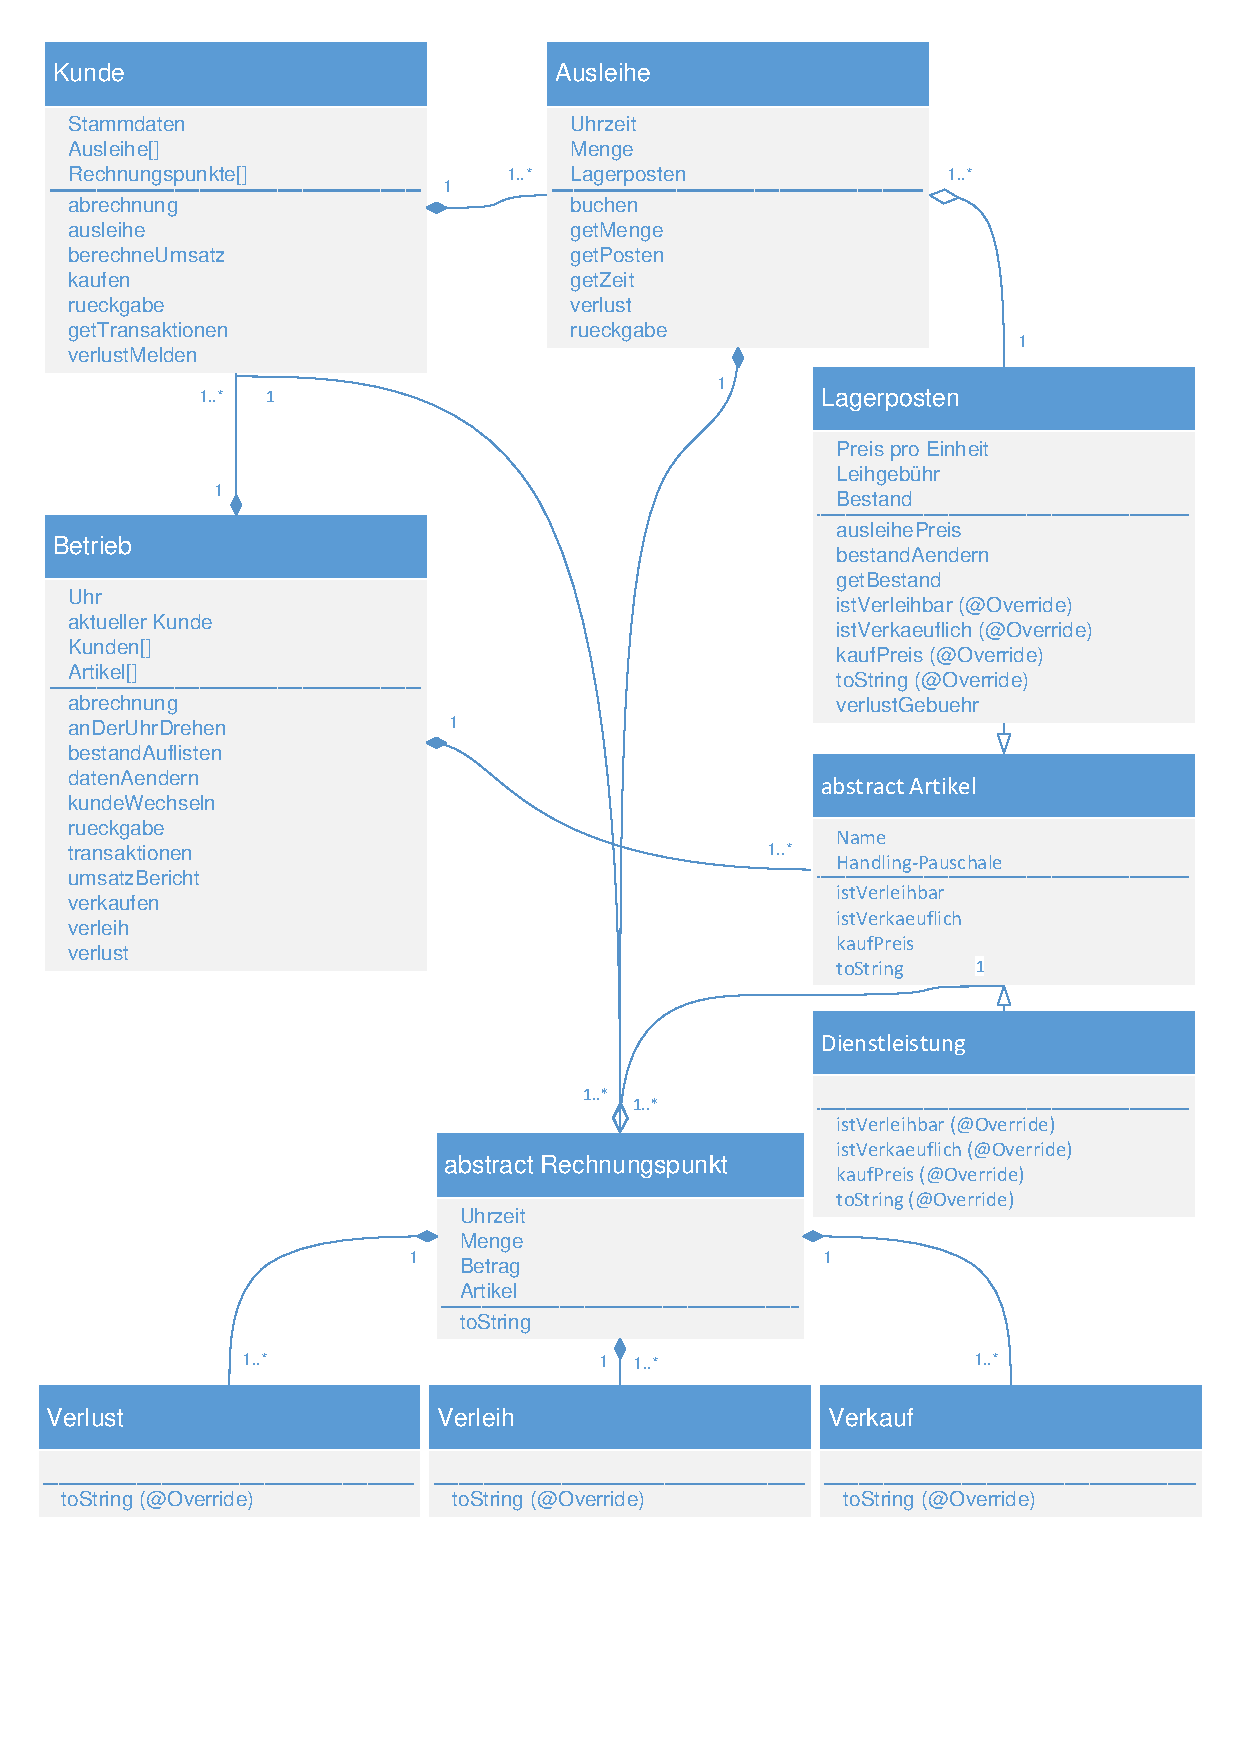
\includegraphics[width=\textwidth]{Klassendiagramm.pdf}
\newpage
\part{Funktionsumfang}
Befehle zur / zum:
\begin{enumerate}
\item Auflistung der aktuell verfügbaren verkäuflichen Gegenstände
\item Auflistung der aktuell verfügbaren  Leihgegenstände
\item Auflistung des gesamten verkäuflichen und verleihbaren Bestands
\item Auflistung der aller Kunden mit ihren Gesamtumsätzen
\item Auflistung aller offenen Transaktionen  und fertigen rechnungspunkte eines Kunden
\item Verkauf eines verfügbaren Objekts
\item Ausleihe eines verfügbaren Objekts für eine prognostizierte Zeitdauer
\item Rückgabe einer vollständigen oder unvollständigen Menge an Objekten
\item Verlustmeldung eines Teiles bzw. der gesamten Ausleihe
\item Abrechnung eines Kunden bei  Rückgabe, Verlust, Kauf oder Nutzung einer Dienstleistung für die entsprechenden Mengen (keine Berücksichtigung von noch ausgeliehenen Gegenständen)
\item Anlegen und Ändern von Kundendaten
\item Wechsel zwischen Kunden
\end{enumerate}
\part{Methodenbeschreibung}
\section{Kunde}
\begin{description}
\item[\{set, get\}\{Name, VorName, ID, Straße, Hausnummer, PLZ, Ort\}]
Holt oder ändert die entsprechenden Werte.
\item[rueckgabe(posten, zeit, menge)]
Bucht eine gegebene Menge eines gegebenen Postens von den Ausleihen des Kunden zurück ins Lager
und stellt die Kosten der Ausleihe dem Kunden in Rechnung.\\
Exception wenn der Posten nicht ausgeliehen war oder die angegebene Menge die Leihmenge übersteigt.
\item[verlustMelden(posten, zeit, menge)]
Streicht eine gegebene Menge eines gegebenen Postens von den Ausleihen des Kunden\\
Exception wenn der Posten nicht ausgeliehen war oder die angegebene Menge die Leihmenge übersteigt.
und stellt dem Kunden die Verlustgebühr in Rechnung.
\item[ausleihe(ausleihe)]
Fügt eine Ausleihe dem Kundenkonto hinzu. Dabei wird diese gebucht.
\item[abrechnung(zeit) $\rightarrow$ RechnungPosten{[]}]
Gibt alle ausstehenden Rechnungspunkte zurück und legt sie damit zu den bearbeiteten Rechnungspunkten.
\item[berechneUmsatz() $\rightarrow$ geld]
Berechnet den gesamten Umsatz, der durch den Kunden verursacht wurde, d. h. der Wert aller bearbeiteten Rechnungspunkte.
\item[getTransaktionen() $\rightarrow$ String{[]}]
Stellt alle Rechungspunkte und bestehenden Ausleihen zusammen.
\item[kaufen(artikel, menge)]
Verkauft (entfernt Bestand) und stellt dem Kunden den Kaufpreis in Rechnung.
\end{description}
\section{Ausleihe}
\begin{description}
\item[buchen()]
Die Ausleihe tritt in Kraft: Entfernt die auszuleihende Menge des Posten aus dem Lager.
\item[getPosten() $\rightarrow$ LagerPosten]
Gibt den Posten der geliehen wird, zurück.
\item[getMenge() $\rightarrow$ menge]
Gibt die ausgeliehende / auszuleihende Menge zurück.
\item[getZeit() $\rightarrow$ zeit]
Gibt die Startzeit der Ausleihe zurück.
\item[verlust(menge) $\rightarrow$ menge]
Annuliert eine bestimmte Menge in der Ausleihe, gibt ggf. die Menge, die von anderen Ausleihen gedeckt wird, zurück.
\item[rueckgabe(menge) $\rightarrow$ menge]
Bucht eine bestimmte Menge zurück, gibt ggf. die Menge, die von anderen Ausleihen gedeckt wird, zurück.
\end{description}
\section{Artikel (abstract)}
\begin{description}
\item[toString() $\rightarrow$ String]
gibt die Daten des Postens, zB in der Form \enquote{<Bestand> x <ID> <Name> (<Einheit>)} als String zurück
\item[istVerkaeuflich() $\rightarrow$ boolean]
Bestimmt ob der Artikel verkäuflich ist.
\item[istVerleihbar() $\rightarrow$ boolean]
Bestimmt ob der Artikel verleihbar ist.
\item[kaufPreis(menge) $\rightarrow$ geld]
Bestimmt den Kaufpreis einer gegebenen Menge des Postens.
\section{Lagerposten}
\item[bestandAendern(menge)]
Ändert den Bestand um die angegebene Menge (positiv oder negativ). \\
Exception wenn Bestand negativ werden würde.
\item[getBestand() $\rightarrow$ geld]
Gibt den aktuellen Lagerbestand zurück.
\item[ausleihePreis(zeit, menge) $\rightarrow$ geld]
Bestimmt die Leihgebühr einer gegebenen Menge des Postens über eine gegebene Zeitspanne.
\item[verlustGebuehr(zeit, menge) $\rightarrow$ geld]
Bestimmt die Gebühr, die bei Verlust einer gegebenen Menge des Postens nach gegebener Zeit entsteht.
\end{description}
\section{Betrieb}
\begin{description}
\item[main(args)]
Hauptmenü
\item[bestandAuflisten(modus)]
listet den Bestand, gefiltert nach Kriterien, die durch modus bestimmt werden (Gesamtbestand, verf. Verkaufsware, verf. Verleihware, oÄ), auf
\item[verkaufen()]
der Verkaufs-Menüpunkt
\item[verleih()]
der Verleih-Menüpunkt
\item[abrechnung(kundenID)]
rechnet alle ausstehenden Rechnungspunkte beim Kunden ab
\item[rueckgabe()]
der Rückgabe-Menüpunkt
\item[verlust()]
der Verlust-Meldungs-Menüpunkt
\item[umsatzBericht()]
listet die Umsätze der Kunden auf
\item[datenAendern(kundenID)]
ändert die Daten eines Kunden (Menü)
\item[transaktionen(kundenID)]
zeigt die Transaktionen eines Kunden an
\item[anDerUhrDrehen(zeit)]
schreitet die Zeit voran
\item[kundeWechseln()]
wechselt den aktiven Kunden
\end{description}
\part{Testfälle}
\begin{enumerate}
\item
Auflistung des Gesamtbestandes zum Kaufen und zum Verleihen.\\
$\Rightarrow$ Liste mit n Elementen zum Verkaufen und n Elementen zum Verleihen
\item
Auflistung des Gesamtbestandes zum Kaufen und zum Verleihen nach einer Änderung um x.\\
$\Rightarrow$ Liste mit n-x bzw. n+x Elementen zum Verkaufen und zum Verleihen
\item
Auflistung des aktuell verfügbaren Bestandes zum Ausleihen und zum Kaufen.
$\Rightarrow$ Liste mit y Elemente unterschiedlich(nach Ausleihe oder Verkauf) bzw. gleich zur Liste des Gesamtbestandes. 
\item
Auflistung des aktuell verfügbaren Bestandes zum Ausleihen und zum Kaufen nach einer Ausleihe bzw. eines Kaufe.
$\Rightarrow$ Liste mit y Elemente unterschiedlich(nach Ausleihe oder Verkauf) bzw. gleich zur Liste des Gesamtbestandes. 
\item
Verleihen von verfügbaren, nicht verfügbaren (die größer sind als die verfügbaren Mengen) und nichtganzzahligen Mengen.
$\Rightarrow$ Führt zu Veränderungen am Bestand der zurzeit verfügbaren Objekten, sofern es verfügbar war 
\item
Verkauf von verfügbaren, nicht verfügbaren (die größer sind als die verfügbaren Mengen) und nichtganzzahligen Mengen.
$\Rightarrow$ Führt zu Veränderungen am Gesamtbestand und am zurzeit verfügbaren Bestand, sofern es verfügbar war
\item
Rückgabe von Mengen, die die Ausleihe übersteigen(sollte nicht möglich sein).
$\Rightarrow$ sollte eine Fehlermeldung ausgeben und keine Ausleihmengen, Rechnungspunkte oder sonstige Daten ändern
\item
Rückgabe testen:
\begin{itemize}
\item vollständig
\item unvollständig 
\item im teilweise oder vollständigen Verlustfall
\end{itemize}
$\Rightarrow$ Veränderungen der Liste aktuell verfügbarer Objekte, macht eine Abrechnung , löscht oder ändert(bei unvollständig) das entsprechende Ausleih-Objekt und den Verweis
\item
Abrechnung testen.
$\Rightarrow$ schafft einen neuen Rechnungspunkt mit den Daten von Objekt Menge, Zeitraum und Kosten
\item
Umsatzliste testen.
$\Rightarrow$ Gibt eine Liste mit einem Eintrag pro Kunden aus, wo die Gesamtsumme der Transaktionen steht
\item
Transaktionen auflisten.
\item
$\Rightarrow$ Gibt eine Liste von n Rechnungspunkten mit Menge, Art, Zeitraum, Preis der Transaktion und Gesamttransaktionenpreis für einen bestimmten Kunden aus
Kundendaten ändern .
$\Rightarrow$ Sollte die entsprechende Änderung speichern und zurückgeben
\item
Neuen Kunden aufnehmen.
$\Rightarrow$ erzeugt ein neues Kundenobjekte, führt zu einem weiteren Eintrag in der Umsatzanzeige
\item
Computer-Mensch Dialog überprüfen (auf Aktionen die möglich sind und welche die nicht möglich sind).
$\Rightarrow$ Fehlermeldungen bei Falscheingabe
\item
Kauf von nicht verkäuflichen Objekten(sollte nicht möglich sein).
$\Rightarrow$ Fehlermeldungen bei Falscheingabe, keine Änderung von Daten(Gesamtbestand, zurzeit verfügbarer Bestand, Rechnungspunkt )
\item
Leih von von nicht verleihbaren Objekten(sollte nicht möglich sein).
$\Rightarrow$ Fehlermeldungen bei Falscheingabe, keine Änderung von Daten(zurzeit verfügbarer Bestand, Ausleihobjekt )
\item
Zeitpunkt in die Vergangenheit ändern bzw. negative Zeitdauer(sollte nicht möglich sein).
$\Rightarrow$ Fehlermeldung, keine Datenänerung, bitte um Neueingabe
\item
Zeitpunkt in die Zukunft ändern.
\item
Differenzberechnung zwischen entliehenem und zurückgegebenen Zeitpunkt
\item
Kunden wechseln
$\Rightarrow$ Gibt eine entsprechende Meldung aus und übergibt einen anderen KundenID-Wert an die Methoden
Programm unterscheidet zwischen Gegenständen und Dienstleistungen
$\Rightarrow$ Bei Dienstleistungen werden keine Änderungen des Gesamt- oder zuzeitverfügbaren Bestandes durchgeführt, keine Verlustpaschale, Leihgebür oder verkaufsgebür  berechnet und in den Rechnungsposten aufgenommen
\item Überprüfung der Berücksichtigung der Handlingpauschale
$\Rightarrow$ handlingpauschale wird bei Verkauf und Verleih bei Rückgabe pro Objekt mitberücksichtigt und in den Rechnungsposten mitaufgenommen, bei Verlust hingegen nicht
\item Toilettenwagen und Frischwasser können nicht verlohren werden
\item Dienstleistungen werden vorher als Rechnungspunkt berechnet
\end{enumerate}
\appendix
\newpage
\part{Eigenständigkeitserklärung}
Wir versichern hiermit, dass wir diese Arbeit selbständig verfasst, keine anderen Quellen und Hilfsmittel
als die angegebenen benutzt und die Stellen der Arbeit, die anderen Werken dem Wortlaut oder dem Sinn nach entnommen sind,
in jedem einzelnen Fall unter Angabe der Quelle als Entlehnung kenntlich gemacht haben.
Das gleiche gilt auch für eingefügte Zeichnungen, Kartenskizzen und Darstellungen.
\begin{itemize}
\item Hameln, \today, \includegraphics{UnterschriftJonaStubbe.png}
\item Hameln, \today, Florian Bussmann	
\item Hameln, \today, Leon Westhof
\end{itemize}
\end{document}
